\documentclass[a4paper]{article}

\usepackage{microtype}
\usepackage{fullpage}
\usepackage{mathtools}
\usepackage{amsfonts}
\usepackage{tikz}
\usepackage{pgfplots}
\usepackage{hyperref}
\usepackage{amsthm}
\usepackage{xcolor}
\usepackage[backend=biber,style=authoryear,maxbibnames=99,hyperref=true]{biblatex}

\addbibresource{references.bib}

\usepgfplotslibrary{fillbetween}
\usetikzlibrary{shapes}
\pgfplotsset{compat=1.17}

\newtheorem{proposition}{Proposition}
\newtheorem{corollary}{Corollary}
\newtheorem{lemma}{Lemma}

\newcommand{\dt}{\mathrm{d}t}
\newcommand{\ds}{\mathrm{d}s}
\newcommand{\E}{\mathbb{E}}

\title{The value of intermediation -- results so far}
\author{Martin Stancsics}

\begin{document}

\maketitle

\begin{abstract}
    This paper proposes a simplified model of two-sided markets aimed at analyzing the shares of total surplus various participants can achieve. Instead of explicitly modelling price structures and entry choices, I use a cooperative approach as a reduced-form model of bargaining outcomes. I show that this technique provides an analytically very tractable way of expressing the profits and surpluses of the agents.
\end{abstract}


\section{Motivation}

The use of solution concepts from cooperative game theory, such as the Shapley-value, to model the outcome of a bargaining process has been a feature of many papers in the industrial organization literature. It is particularly prevalent in articles dealing with issues related to integration and mergers \parencite[e.g.][]{hart1990property,segal2003collusion,inderst2003bargaining,montez2007downstream}. This is in part motivated by the appealing properties of the resulting distributions, their tractability, but also by the long line of studies showing that various bargaining procedures lead to such outcomes. For example, \textcite{gul1989bargaining,winter1994demand,hart1996bargaining,inderst2003bargaining,} or, perhaps most relevant to this paper, \textcite{stole1996intra} all propose various extensive-form bargaining games in which the expected outcomes correspond to players' Shapley-values.

A common feature of the aforementioned papers is that they involve models with a finite number of agents. However, as is often the case in economics, the infinite-player approximations might turn out to be more tractable while retaining the main conclusions of the finite models from which they arise. Indeed, in the case of cooperative games with non-atomic players, the axiomatic and asymptotic approaches both give rise to the same value\footnote{On the appropriate subspace of non-atomic games.} \parencite{aumann2015values}, which is furthermore analytically simple and readily interpretable. An economic application of this theory can be found in \textcite{billera1978internal}.

Beyond games with no atoms, economists are often interested in situations characterized by a relatively small number of large players and numerous individually rather insignificant ones. The continuous analogue of them are called oceanic games, in which the set of players consists of a finite number of atoms and an ocean made up of a continuum of fringe players. While the axiomatic characterization of the value on such games has not been particularly fruitful,\footnote{\textcite{hart1973values} shows that the usual axioms do not characterize a unique value in general.} \textcite{fogelman1980asymptotic} demonstrates that the asymptotic approach works well on a large subset of them.

Despite this positive result, and their analytical tractability, oceanic games are utilized by hardly any papers in economics. One of the few such examples is \textcite{levy1997individual}, applying it to the problem of wage bargaining. In the following, I propose an oceanic game with the main feature that the large player(s) is indispensable for creating value. Such a model can apply, for example, to upstream-downstream supply chains, or platforms connecting two sides of a market. I demonstrate that the values of the players in those models are described by easily interpretable and visualizable expressions. Furthermore, the results are simple enough that these games can be embedded into more complex models, for example, as the second stage of a sequential game \parencite[as in e.g.][]{montez2007downstream}. Just as importantly, the outcomes are in line with one's intuitive expectations of bargaining outcomes in such situations.


\section{One-sided case}

Imagine a cooperative game with two types of players: a major player $P$ and $n$ smaller players. I.e., $N = \{P, A_1, \dots, A_n\}$. Assume that (1) no coalition of players can achieve a positive value without the participation of $P$ and (2) players $A_i$ are identical. Let $n_T(S)$ denote the number of players of type $T$ in coalition $S$. Then, the value $S \subset N$ can achieve is the following:
\begin{align*}
    v(S) = \begin{cases}
        0                              & \text{if } P \notin S \\
        f\left(\frac{n_A(S)}{n}\right) & \text{otherwise}.
    \end{cases}
\end{align*}
One can think of this setting as a (one-sided) platform and a number of potential entrants.

\begin{proposition}
    The game $(N, v)$ is monotone and superadditive if and only if $f$ is increasing and $f(0) \geq 0$. % It is supermodular if and only if $f$ is convex.
\end{proposition}
\begin{proof}
    Monotonicity is evident. For superadditivity, note that for any $S, T$ such that $S \cap T = \emptyset$, $P \notin S$ or $P \notin T$. WLOG assume it is the latter, therefore $v(T) = 0$. As a result, $v(S) + v(T) = v(S) \leq v(S \cup T)$ holds if and only if $(N, v)$ is monotone.
\end{proof}
In the following, let us assume that the assumptions required for monotonicity are always satisfied. It ensures that the games are of bounded variation, and thus the main theorem in \textcite{fogelman1980asymptotic} applies: asymptotic value coincides with the axiomatic one using the uniform distribution for the latter. \textcolor{red}{Note: I realize that this paragraph is somewhat vague and needs explanation. However, for the current set of results, I do not rely on said theorem. If I end up using it later, I will expand on this part.}

Let $\varphi_P^n$ denote the Shapley-value of player $P$ in the case of $n$ players of type $A$. The following proposition demonstrates the main idea of this paper: even as the number of fringe players goes to infinity, the Shapley-value of the platform does not converge to $f(1)$. This in turn implies that the aggregated Shapley-values of the fringe remain positive even in the limit.
\begin{proposition}
    \label{prop:one_sided}
    Let $f$ be continuous on [0, 1]. Then
    \begin{align*}
        \varphi_P^\infty = \lim_{n \to \infty} \varphi_p^n = \int_0^1 f(t) \dt .
    \end{align*}
\end{proposition}
\begin{proof}
    For a permutation of players $R$, let us denote the players preceding $i$ by $\mathcal{P}_i^R$. The value of player $P$ is their expected marginal contribution averaged over all permutations of $N$:
    \begin{align*}
        \varphi_P^n = \frac{1}{(n+1)!} \sum_R v(\mathcal{P}_P^R \cup \{i\}) - v(\mathcal{P}_P^R)
    \end{align*}
    First, note that $v(\mathcal{P}_P^R) = 0$ for any permutation, as no coalition can achieve a positive value without player $P$. Furthermore, using the fact that all agents of type $A$ are identical implies that $v(\mathcal{P}_P^R \cup \{i\})$ only depends on the number of agents in the coalition. More precisely, 
    \begin{align*}
        v(\mathcal{P}_P^R \cup \{i\}) = f(n_A(\mathcal{P}_P^R \cup \{i\}) / n) = f(|\mathcal{P}_P^R| / n).
    \end{align*}
    Finally, the set of permutations in which the number of players preceding $P$ is $k$ is independent of $n$, i.e.
    \begin{align*}
        \{R \mid |\mathcal{P}_P^R| = k\} = n! \quad \forall\, k.
    \end{align*}
    Putting all the above together, the value of player $P$ can be expressed as
    \begin{align*}
        \varphi_P^n &= \frac{1}{(n+1)!} \sum_{k=0}^n n! f(k / n) \\
        &= \frac{1}{n+1} \sum_{k=0}^n f(k / n) \\
        &= \frac{n}{n+1} \underbrace{\frac{1}{n} \sum_{k=0}^{n-1} f(k / n)}_{=S_n} + \frac{1}{n+1} f(1).
    \end{align*}
    $S_n$ are just the left Riemann-sums of function $f$ on the interval $[0, 1]$. Therefore, if $f$ is continuous (and thus Riemann-integrable), then $S_n \to \int_0^1 f(t)$, and thus
    \begin{align*}
        \lim_{n \to \infty} \varphi_P^n &= \lim_{n \to \infty} \frac{1}{n+1} \sum_{k=1}^n f(k / n) \\
        &= \lim_{n \to \infty}\underbrace{\frac{n}{n+1}}_{\to 1} \frac{1}{n} \sum_{k=0}^{n-1} f(k / n) + \underbrace{\frac{1}{n+1} f(1)}_{\to 0} \\
        &= \int_0^1 f(t) \dt .
    \end{align*}
\end{proof}

The above proposition is not surprising in light of \textcite{fogelman1980asymptotic}: the limit is just the expected marginal contribution of the single atomic player, with said player being placed in the order according to the uniform distribution. Nevertheless, even this simple result has a compelling geometric interpretation, and gives rise to a couple of interesting corollaries, detailed below.

\begin{corollary}
    The aggregated Shapley-value of the fringe (alternatively, the per-unit Shapley-value of the fringe) is
    \begin{align*}
        \varphi_A^\infty = f(1) - \int_0^1 f(t) \dt.
    \end{align*}
    Furthermore, if $f$ is differentiable on $[0, 1]$, Then the value of the fringe can also be expressed as
    \begin{align*}
        \varphi_A^\infty = \int_0^1 t f'(t) \dt.
    \end{align*}
\end{corollary}
\begin{proof}
    The first equality comes from the efficiency of the Shapley-value. The values of all players sum up to $f(1)$ for all $n \in \mathbb{N}$, therefore
    \begin{align*}
        \lim_{n \to \infty} \sum_{i=1}^n \varphi_{A_i}^n = \lim_{n \to \infty} (1 - \varphi_P^n ) = 1 - \int_0^1 f(t).
    \end{align*}
    The second can be obtained by integration by parts:
    \begin{align*}
        \int_0^1 t f'(t) \dt = tf(t) \mid_0^1 - \int_0^1 f(t) \dt = f(1) - \int_0^1 f(t) \dt
    \end{align*}
\end{proof}

It is already apparent from Figure \ref{fig:one_sided} that (for fixed $f(0)$ and $f(1)$) player $P$ gets a larger share of the surplus when $f(t)$ is large even for small values of $t$. It corresponds to the case when only a small fraction of the fringe is needed to create most of the surplus (e.g. their products are substitutes of each other). This result aligns with our natural intuition that player $P$ has a better bargaining position in this case, than if only coalitions with most of the fringe firms could obtain high values.

\begin{figure}
    \centering
    \caption{Distribution of value between player $P$ and the fringe}
    \label{fig:one_sided}
    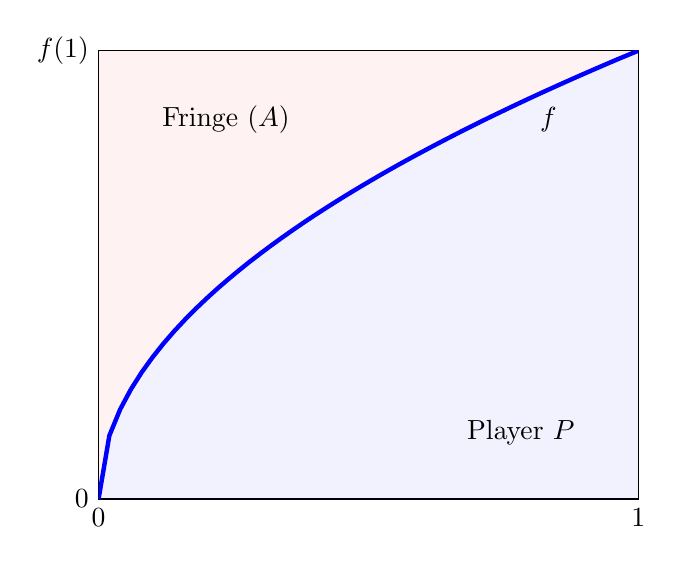
\begin{tikzpicture}
        \begin{axis}[xmin=0, xmax=1, ymin=0, ymax=1, samples at={0, 0.02, ..., 0.98, 1},
                xtick={0, 1}, ytick={0}, extra y ticks={1},  extra y tick style={yticklabel={$f(1)$}}]
            \addplot[name path=f, blue,ultra thick] {x^0.5};
            \node[anchor=north west] at (axis cs: .8, .8^0.5) {$f$};
            \path[name path=bottom] (axis cs:0,0) -- (axis cs:1,0);
            \path[name path=top] (axis cs:0,1) -- (axis cs:1,1);

            \addplot [fill=blue, fill opacity=0.05] fill between [of=f and bottom];
            \addplot [fill=red, fill opacity=0.05] fill between [of=f and top];

            \node[anchor=north west] at (axis cs: .1, .9) {Fringe ($A$)};
            \node[anchor=south east] at (axis cs: .9, .1) {Player $P$};
        \end{axis}
    \end{tikzpicture}
\end{figure}

\begin{corollary}
    $\varphi_P^\infty < f(1)$ and $\varphi_A^\infty > 0$ for any $f$ that is not constant.
\end{corollary}
\begin{proof}
    If $f$ is monotone increasing, then $f(0) \leq \int_0^1 f(t) \dt \leq f(1)$. The inequalities become strict if $f$ is not constant on the whole interval.
\end{proof}

This proposition gives credence to using asymptotics to model situations with a finite, albeit large number of players. Even though the individual share of each $A_i$ vanishes as their number goes to infinity, their total value converges to a positive value.


\subsection{Weighted Shapley-values}

Imagine a general non-cooperative game $(N, v)$ with $N = \{1, \dots, n\}$. Assume that, in addition to the value function $v : 2^n \to \mathbb{R}$, the game is also endowed with a weight system $\lambda \in \mathbb{R}^n$. These weights can be thought of as measures of innate bargaining power \parencite{shapley1953additive}, not reflected in the value function. Further support for this interpretation can be found in \textcite{hart1996bargaining}, demonstrating that in a certain alternating offer bargaining game, weights are related to the probability of each player making the offer.\footnote{For example, only one player having a positive value corresponds to them making take it or leave it offers.}

For my purposes, it is sufficient to deal with the case of simple weights. I.e., assume that there is at most one player with zero weight. I make use of the fact that weighted Shapley values can be calculated by weighting the permutations by the probabilities arising from the following sequential entry procedure \parencite{kalai1987weighted}. Start adding players from the end. The probability of player $i$ being the last amongst the set of remaining players $R$ is $\lambda_i / \sum_{j \in R} \lambda_j$. This yields a well-defined probability for each permutation of players.

Getting back to the game at hand, let the weights of players of type $A$ and $P$ be 1 and $\lambda$, respectively. Let $X_n$ be a random variable representing the number of players before $P$ when players are ordered according to the above procedure. Then, the probability of player $P$ having at most $k$ players of type $A$ before themselves is simply
\begin{align*}
    \Pr{X_n \leq k} = \prod_{j=k+1}^n \frac{j}{j + \lambda} .
\end{align*}
The following lemma establishes the continuous analogue of this statement.
\begin{lemma}
     As $n \to \infty$, $X_n \xrightarrow[]{\mathrm{d}} X$ with the cdf $G_X(t) = \lambda^t$. Consequently, the corresponding probability density function is $g(t) = \lambda t^{\lambda - 1}$.
\end{lemma}
\begin{proof} \textcolor{red}{(Might have to fix sum indices)} \\
    The probability of $P$ having at most fraction $t$ of the other players before itself is
    \begin{align*}
        \Pr(X_n \leq nt) &= \Pr(X_n \leq nt ) \\
        &= \prod_{j = nt + 1}^n \frac{j}{j + \lambda} \\
        &= \exp \Bigg( \underbrace{\sum_{j = nt + 1}^n \log(j) - \log(j+\lambda)}_{\equiv S_n} \Bigg).
    \end{align*}
    Taking limits,
    \begin{align*}
        \lim_{n \to \infty} S_n &= \lim_{n \to \infty} \sum_{j = nt + 1}^n \log(j) - \log(j+\lambda) \\
        &= \lim_{n \to \infty} \sum_{i = 1}^{n - nt} \log(nt + i) - \log(nt + i + \lambda) \\
        &= \lim_{n \to \infty} \frac{1}{n - nt} \sum_{i = 1}^{n - nt} \frac{\log \left( t + \frac{i}{n - nt} \right) - \log \left( t + \frac{i}{n - nt} + \frac{\lambda}{n - nt} \right)}{1 / (n - nt)}
    \end{align*}
    Let
    \begin{align*}
        \Delta_n(s) = \frac{\log \left( s \right) - \log \left( s + \frac{\lambda}{n - nt} \right)}{1 / (n - nt)}
    \end{align*}
    By lemma \ref{lemma:log_convergence}, 
    \begin{align*}
        \Delta_n \xrightarrow[]{\mathrm{u}} \lambda \frac{\mathrm{d}}{\mathrm{d}s}log(s) = -\frac{\lambda}{s}
    \end{align*}
    on the compact interval $[t, 1]$ for any $t > 0$ ($\xrightarrow[]{\mathrm{u}}$ denotes uniform convergence).
    
    Then, by lemma \ref{lemma:integral_convergence}, we have that
    \begin{align*}
        \lim_{n \to \infty} S_n &= \lim_{n \to \infty} \frac{1}{n-nt} \sum_{i=1}^{n-nt} \Delta_n \left( t + \frac{i}{n - nt} \right) \\
        &= \int_t^1 (\lim_{n \to \infty} \Delta_n)(s) \ds \\
        &= \int_t^1 \lim_{n \to \infty} -\frac{\lambda}{s} \ds \\
        &= \lambda \log{t}
    \end{align*}

    Substituting $\lim_{n \to \infty} S_n$ into the original equation yields
    \begin{align*}
        \lim \Pr \left( \frac{X_n}{n} \leq t \right) &= \exp \Bigg( \lim_{n \to \infty} \sum_{j = nt + 1}^n \log(j) - \log(j+\lambda) \Bigg) \\
        &= \exp(\lambda \log(t)) \\
        &= t^\lambda.
    \end{align*}

    For $t=0$, simply observe that
    \begin{align*}
        \lim_{n \to \infty} \prod_{j = 1}^n \frac{j}{j + \lambda} = 0 = 0^\lambda.
    \end{align*}
\end{proof}


Finally, the weighted Shapley-value of player $i$ can be expressed as the expected marginal contribution of that player where the permutations are weighted according to the previous distribution.
\begin{proposition}
    \label{prop:one_sided_weighted}
    Let $f(t)$ be continuous on $[0, 1]$. Then
    \begin{align*}
        \varphi_P(\lambda, \infty) = \int_0^1 g(t) f(t) \dt
    \end{align*}
    where $g(t) = \lambda t^{\lambda - 1}$.
\end{proposition}
\begin{proof}
    The weighted value of player $P$ is its expected contribution across all permutations, with each permutation weighted by its probability of occurring.
    \begin{align*}
        \varphi_P^{n, \lambda} = \sum_R \Pr(R) [v(\mathcal{P}_P^R \cup \{i\}) - v(\mathcal{P}_P^R)]
    \end{align*}
    As before, using the fact that fringe players are identical, this can be rephrased as
    \begin{align*}
        \varphi_P^{n, \lambda} &= \sum_{k=0}^n \Pr(R) f(k/n) \\
        &= \E[f(X_n / n)]
    \end{align*}
    where $X_n$ is defined as above. $f$ is continuous, and therefore bounded on the compact set $[0, 1]$. As a consequence, $\frac{X_n}{n} \xrightarrow[]{\mathrm{d}} X$ implies $\E[f(X_n / n)] \to \E[f(X)]$, which in turn gives
    \begin{align*}
        \lim_{n \to \infty} \varphi_P^{n, \lambda} &= \lim_{n \to \infty} \E[f(X_n / n)] \\
        &= \E[f(X)] \\
        &= \int_0^1 f(t) \mathrm{d}G(t) \\
        &= \int_0^1 g(t)f(t) \dt
    \end{align*}
    where $G(t)$ and $g(t)$ are the cdf and pdf of X, respectively.
\end{proof}

\begin{corollary}
    $\varphi_P(\lambda, \infty)$ is increasing in $\lambda$ unless $f$ is constant.
\end{corollary}
\begin{proof}
    Let $X$ and $X'$ be random variables with cdfs $G_X = t^\lambda$ and $G_{X'}t^{\lambda'}$, respectively. For any $\lambda < \lambda'$, $t^\lambda > t^{\lambda'} \forall t \in [0, 1]$, meaning that $X'$ first-order stochastically dominates $X'$. As a result, for any monotonically increasing $f$,
    \begin{align*}
        \int_0^1 g_X(t)f(t) \dt = \E[f(X)] \leq \E[f(X')] = \int_0^1 g_{X'}(t)f(t)
    \end{align*}
    with strict inequality unless $f$ is constant almost everywhere. As $f$ is continuous, the latter is equivalent to $f$ being constant on the whole $[0, 1]$ interval.
\end{proof}

The following proposition supports the interpretation of weights as bargaining power, as a higher weight corresponds to a higher Shapley-value in this game.\footnote{This would not necessarily have to be the case, as demonstrated by \textcite{owen1968communications}.}

\begin{corollary}
    If the weight of player $P$ goes to infinity (zero), its weighted Shapley value converges to $f(1)$ ($f(0)$).
\end{corollary}
\begin{proof}
    As $\lambda \to 0$, $X$ converges to the degenerate random variable $X_0$ for which $\Pr(X_0 = 0) = 1$. As a consequence, the expected value of $f(X)$ converges to $\E[f(X_0)] = f(0)$. $\lim_{\lambda \to \infty} \varphi^{\infty, \lambda}_P = f(1)$ can be shown along the same lines.
\end{proof}

\subsection{Multiple platforms}

Imagine that there are $m$ players of type $P$ which are perfect substitutes of each other. That is, the fringe players still need a platform to achieve any value, but it does not matter which or how many platforms are available for them. Specifically, the value function for coalition $S$ is the following:
\begin{align*}
    v(S) = \begin{cases}
        0                              & \text{if } n_P(S) = 0 \\
        f\left(\frac{n_A(S)}{n}\right) & \text{otherwise}.
    \end{cases}
\end{align*}

% \begin{proposition}
%     The game is monotone, supermodular and convex if $f$ is increasing and convex
% \end{proposition}
\textcolor{red}{Note: I have to think more about how to describe this situation in the language of cooperative game theory. The issue is that, for example, the value of $\{P_1, A_1\}$ depends on whether $\{P_2, A_2\}$ also decides to form a coalition and enter the market.}

\begin{proposition}
    The limit of the Shapley-value (as $n \to \infty$) of each player of type $P$ is
    \begin{align*}
        \varphi_{P_i}^{\infty, m} = \int_0^1 (1-t) ^ {m-1} f(t) \dt .
    \end{align*}
\end{proposition}
\begin{proof}
    \label{prop:one_sided_multiple}
    First, let us rewrite the expected marginal contribution of player $P_i$ in the following way:
    \begin{align*}
        \varphi_{P_i}^{n, m} &= \frac{1}{(n+m)!} \sum_R v(\mathcal{P}_{P_i}^R \cup \{i\}) - v(\mathcal{P}_{P_i}^R) \\
        &= \frac{1}{(n+m)!} \left[ \sum_{\{R | n_P(\mathcal{P}_{P_i}^R = 0)\}} \left[v(\mathcal{P}_{P_i}^R \cup \{i\}) - v(\mathcal{P}_{P_i}^R)\right] + \sum_{\{R | n_P(\mathcal{P}_{P_i}^R > 0)\}} \left[v(\mathcal{P}_{P_i}^R \cup \{i\}) - v(\mathcal{P}_{P_i}^R)\right] \right]
    \end{align*}
    Next, make use of the fact that the marginal contribution of a platform is zero if another platform is already present, and only depends on the number of fringe firms otherwise.
    \begin{align*}
        \varphi_{P_i}^{n, m} &= \frac{1}{(n+m)!} \sum_{\{R | n_P(\mathcal{P}_{P_i}^R = 0)\}} f (\mathcal{P}_{A}^R / n) \\
        &= \frac{1}{(n+m)!} \sum_{k=0}^n |\{R | n_A(\mathcal{P}^R_{P_i} = k) \text{ and } n_P(\mathcal{P}^R_{P_i} = 0)\}| f(k/n)
    \end{align*}
    Finally, notice that, while the permutations with $k$ fringe agents before $P_i$ does not depend on $k$, amongst those, the number of permutations with no platform before $P_i$ does depend on it. In particular,
    \begin{align*}
        |\{R | n_A(\mathcal{P}^R_{P_i} = k) \text{ and } n_P(\mathcal{P}^R_{P_i} = 0)\}| &= \frac{n!(n+m-k-1)!}{(n-k)!}
    \end{align*}
    and
    \begin{align*}
        \varphi_{P_i}^{n, m} &= \sum_{k=0}^n \frac{n!(n+m-k-1)!}{(n+m)!(n-k)!} f(k/n) \\
        &= \sum_{k=0}^n \frac{(n-k+1)(n-k+2) \dots (n-k+m-1)}{(n+1)(n+2) \dots (n+m)} f(k/n) \\
        &= \frac{1}{n+1}\sum_{k=0}^n \underbrace{\frac{(n(1-k/n)+1)(n(1-k/n)+2) \dots (n(1-k/n)+m-1)}{(n+2) \dots (n+m)} f(k/n)}_{S_n}
    \end{align*}
    For any $t = k/n \in [0, 1]$, 
    \begin{align*}
        S_n(t) \to (1-t)^{m-1}f(t) \equiv S(t).
    \end{align*}
    Furthermore, it is simple to verify that this convergence is uniform, and that $S_n$ and $S$ are all continuous functions. By Dini's theorem, the former properties imply that $S_n \xrightarrow[]{\mathrm{u}} S$ uniformly on $[0, 1]$.

    The conclusion of the proof is similar to that of proposition \ref{prop:one_sided}:
    \begin{align*}
        \lim_{n \to \infty} \varphi_{P_i}^{n, m} &= \lim_{n \to \infty} \underbrace{\frac{n}{n+1}}_{\to 1} \sum_{k=0}^{n-1} S_k(k/n) + \underbrace{\frac{1}{1+n}S(1)}_{\to 0} \\
        &= \lim_{n \to \infty} \sum_{k=0}^{n-1} S_k(k/n) \\
        &= \int_0^1 (1-t)^{m-1} f(t) \dt
    \end{align*}
    with the last equality supported by lemma \ref{lemma:integral_convergence}.
\end{proof}

As with proposition \ref{prop:one_sided}, this result also has a probabilistic interpretation, and could have been obtained directly from the oceanic game. Let the location of the $m$ atoms be $t_1, \dots, t_m$, distributed independently and uniformly on the unit cube. The expected marginal contribution of $t_i$ is only positive whenever it is the first amongst the major players. That is, for any $t_i$, the probability if $P_i$ being the first is related to the cdf of the first order statistic from $n-1$ independent uniform distributions: $1 - (1-t)^{m-1}$.

\begin{corollary}
    The per-unit Shapley-value of the fringe is
    \begin{align*}
        \varphi_A(k, \infty) = 1 - m\int_0^1 (1-t) ^ {m-1} f(t) \dt = \int_0^1 [1 - (1-t)^m] f'(t) \dt .
    \end{align*}
\end{corollary}
\begin{proof}
    The allocation is efficient for all $n \in \mathbb{N}$, therefore efficient in the limit, as well. The second equality can be obtained by integration by parts.
\end{proof}

The following corollary again demonstrates that the predicted outcomes confirm intuitions. As the major players become more and more substitutable, the portion of the surplus they can capture decreases, and the aggregated value of the fringe increases.

\begin{corollary}
    Let $\varphi_{P}^{\infty, m} = m\varphi_{P_i}^{\infty, m}$ denote the aggregated values of players of type $P$. $\varphi_{P}^{\infty, m}$ is decreasing in $m$ and $\varphi_{A}^{\infty, m}$ is increasing in $m$ unless $f$ is constant.
\end{corollary}
\begin{proof} \textcolor{red}{(Assuming $f$ is continuously differentiable -- will have to relax this)}
    $f'(t)$ is non-negative, so $[1 - (1-t)^m] f'(t)$ is increasing in $m$ $\forall t \in [0, 1]$. As a consequence, $\varphi_A^{n, \infty}$ is also increasing in $m$ if $f'(t)$ is positive on some interval or, $f(t)$ is not constant. Conversely, $\varphi_{P}^{\infty, m} = 1 - \varphi_{A}^{\infty, m}$ is decreasing in $m$.
\end{proof}

\section{Two-sided case}

\textcolor{red}{\large No proofs or changes in this section. The next new results are in the appendix.}

Now imagine that, in addition to player $P$, there are two types of smaller players: $\{A_1, \dots, A_n\}$ and $\{B_1, \dots, B_n\}$. As before, $P$ is necessary for any coalition to have a positive value, and the small players are identical within their groups. I.e., the set of players and the characteristic function of the game are the following: $N = \{P, A_1, \dots, A_n, B_1, \dots, B_n\}$ and
\begin{align*}
    v(S) = \begin{cases}
        0                                                & \text{if } P \notin S \\
        f\left(\frac{n_A(S)}{n}, \frac{n_A(S)}{n}\right) & \text{otherwise}.
    \end{cases}
\end{align*}

\begin{proposition}
    The game $(N, v)$ is monotone and superadditive if and only if $f$ is increasing in both arguments.
\end{proposition}

Furthermore, the limits of the Shapley-values (as $n \to \infty$) of the various players turn out to be analytically tractable and nicely interpretable.

\begin{proposition}
    Let $f(a, b)$ be continuous everywhere on $[0, 1]^2$. Then,
    \begin{align*}
        \varphi_P^\infty & = \int_0^1 f(t, t) \dt                                 \\
        \varphi_A^\infty & = \int_0^1 t \frac{\partial f(t, t)}{\partial a} \dt   \\
        \varphi_B^\infty & = \int_0^1 t \frac{\partial f(t, t)}{\partial b} \dt .
    \end{align*}
\end{proposition}

That is, the value of the grand coalition can be decomposed into the Shapley-values of its members signifying their expected marginal contributions in the following way:
\begin{align*}
    f(1, 1) = \underbrace{\int_0^1 f(t, t) \dt}_{\text{ player } P} + \underbrace{\int_0^1 t \frac{\partial f(t, t)}{\partial a} \dt}_{\text{players } A} + \underbrace{\int_0^1 t \frac{\partial f(t, t)}{\partial b} \dt}_{\text{players } B}
\end{align*}


\subsection{Multiple platforms}

Again, assume that there are $k$ players of type $P$ which are perfect substitutes of each other.

\textbf{Note:} As in the previous case, I have to think more about how interpret the value function here. For now, let me just show the limit of the limits of the Shapley-values assuming that
\begin{align*}
    v(S) = \begin{cases}
        0                                                & \text{if } P_i \notin S \; \forall \, i = 1, \dots, k \\
        f\left(\frac{n_A(S)}{n}, \frac{n_B(S)}{n}\right) & \text{otherwise}.
    \end{cases}
\end{align*}

\begin{proposition}
    The unit Shapley-values of the various types of players are
    \begin{align*}
        \varphi_{P_i}(k, \infty) & = \int_0^1 (1-t)^{k-1} f(t, t) \dt                                 \\
        \varphi_A(k, \infty)     & = \int_0^1 [1 - (1-t)^k] \frac{\partial f(t, t)}{\partial a} \dt   \\
        \varphi_B(k, \infty)     & = \int_0^1 [1 - (1-t)^k] \frac{\partial f(t, t)}{\partial b} \dt .
    \end{align*}
\end{proposition}

\begin{corollary}
    Let $\varphi_{P}(k, \infty) = k\varphi_{P_i}(k, \infty)$ denote the aggregated Shapley-values of players of type $P$. Then $\varphi_{P}(k, \infty)$ is decreasing in $k$ and $\varphi_{A}(k, \infty)$, $\varphi_{B}(k, \infty)$ is increasing in $k$ unless $f$ is constant.
\end{corollary}


\appendix

\section{Miscellaneous lemmas}

\begin{lemma}
    \label{lemma:log_convergence}
    Let 
    \begin{align*}
        \Delta_n(s) &= \frac{\log(s + 1/n) - \log(\lambda)}{n}, \\
        \Delta(s) &= \frac{1}{s}.
    \end{align*}
    Then $\Delta_n \xrightarrow[]{\mathrm{u}} \Delta$ uniformly on $[t, 1]$ for any $t > 0, \lambda > 0$.
\end{lemma}
\begin{proof}
    First, note that $\Delta_n$ and $\Delta$ are all continuous functions. Then, following the standard proof for $\frac{\mathrm{d}}{\mathrm{d}s}log(s) = \frac{1}{s}$ rewrite $\Delta_n(s)$ as
    \begin{align*}
        \Delta_n(s) &= \frac{\log(s + 1/n) - \log(\lambda)}{n} \\
        &= \log \left( 1 + \frac{1}{sn} \right) ^ n .
    \end{align*}
    It is well known that $\left( 1 + \frac{1}{sn} \right) ^ n$ is monotone increasing in $n$ and converges to $\exp (1/s)$. Therefore, the pointwise convergence of $\Delta_n(s) \to \Delta(s)$ is also monotone.

    Finally, by Dini's theorem, the monotone pointwise convergence of a sequence of continuous functions to a continuous function on a compact set implies uniform convergence on that set.
\end{proof}

\begin{lemma}
    \label{lemma:integral_convergence}
    Let $f_n, f: [a, b] -> \mathbb{R}$ be Riemann-integrable functions with $f_n \xrightarrow[]{\mathrm{u}} f$ uniformly. Then,
    \begin{align*}
        \lim_{n \to \infty} \frac{b-a}{n} \sum_{k=1}^n f_n \left( a + \frac{b-a}{n} \right) = \int_0^1 f(t) \dt.
    \end{align*}
\end{lemma}
\begin{proof}
    \begin{align*}
        &\lim_{n \to \infty} \frac{b-a}{n} \sum_{k=1}^n f_n \left( a + \frac{b-a}{n} \right) \\
        &= \lim_{n \to \infty} \frac{b-a}{n} \left[ \sum_{k=1}^n f \left( a + \frac{b-a}{n} \right) + \sum_{k=1}^n \left( f_n \left( a + \frac{b-a}{n} \right) - f \left( a + \frac{b-a}{n} \right) \right) \right] \\
        &= \int_a^b f(t) \dt + \lim_{n \to \infty} \frac{b-a}{n}\sum_{k=1}^n \left( f_n \left( a + \frac{b-a}{n} \right) - f \left( a + \frac{b-a}{n} \right) \right) \\
        &\leq \int_a^b f(t) \dt + \lim_{n \to \infty} \frac{b-a}{n}\sum_{k=1}^n \left| f_n \left( a + \frac{b-a}{n} \right) - f \left( a + \frac{b-a}{n} \right) \right| \\
        &\leq \int_a^b f(t) \dt + \lim_{n \to \infty} \frac{b-a}{n}\sum_{k=1}^n \sup_{t \in [a, b]} \left| f_n(t) - f(t) \right| \\
        &= \int_a^b f(t) \dt + (b-a) \underbrace{\lim_{n \to \infty} \sup_{t \in [a, b]} \left| f_n(t) - f(t) \right|}_{=0 \text{ due to uniform convergence}} \\
        &= \int_a^b f(t) \dt
    \end{align*}
\end{proof}


\section{References}

\printbibliography

\end{document}